% Copyright 2026 Sreeram Anil
% SPDX-License-Identifier: CC-BY-4.0
% =============================================================================
%  Strong tracking filter (suboptimal fading factor)
% =============================================================================
\chapter{Strong tracking filter (STF)}
\label{ch:stf}

\section*{At a glance}
\begin{tabular}{@{}l>{\raggedright\arraybackslash}p{0.76\textwidth}@{}}
Family & Adaptive Kalman \\
Header & \texttt{include/estkit/filters/stf.hpp} \\
Registered name & \texttt{STF} \\
State dimension & $n_x = 4$ (cell model) --- generic in $n_x, n_u, n_y$ \\
Cost per step & EKF $+$ one $n_x\times n_x$ scale-and-add $+\,\mathcal{O}(n_y^2 n_x)$; $\approx 530$\,ns/step, no heap \\
Primary references & \cite{zhoufrank1996stf,xia1994adaptive,jwo2007fuzzy,simon2006,jazwinski1970} \\
\end{tabular}

\section{Motivation and aerospace/BMS relevance}
A converged Kalman filter is a very confident object.  After a few hundred samples $\Pplus$ has
settled at its steady-state value, the gain is small, and the filter's estimate is dominated by its
own model.  That is exactly what one wants when the model is right --- and exactly what one does not
want when it is not.  A sudden manoeuvre, a change of the vehicle's mass, a cell whose internal
resistance has grown by $25\,\%$ since the model was identified: in every case the innovation
sequence stops being white and starts carrying a systematic component that the filter, having
already decided that it knows the state, largely ignores.  Anderson and Moore
\cite[Sec.~4.4]{andersonmoore1979} call the resulting slow, monotone error growth \emph{divergence
through model mismatch}; it is the single most common failure mode of Kalman filters in the field.

Zhou and Frank \cite{zhoufrank1996stf} proposed a direct cure.  They keep the minimum-variance
requirement of the Kalman filter but \emph{add} a second requirement: the innovation sequence must
be orthogonal at all non-zero lags, that is, white.  Whiteness of the innovations is the classical
signature of an optimal filter (Kailath's innovations representation, \cite[Ch.~9]{kailath2000});
if the residuals are still correlated, information remains in them that the filter has failed to
extract.  Zhou and Frank enforce the second requirement, suboptimally, by inserting a single scalar
\emph{fading factor} $\lambda_k\ge 1$ in front of the propagated part of the prediction covariance.
The effect is that the filter's memory is shortened automatically and only when the innovations say
it must be, which is why the method is called \emph{strong tracking}: it tracks abrupt changes
strongly while degenerating to the ordinary EKF when nothing is wrong.

The STF is widely used in fault detection and isolation, in manoeuvring-target tracking, and in
GNSS/INS integration where it is often combined with a fuzzy supervisor \cite{jwo2007fuzzy}.  The
closely related "adaptive fading Kalman filter" of Xia et al.\ \cite{xia1994adaptive} uses the same
inflation with a differently computed factor.  In a BMS the natural targets are an aged cell whose
parameters no longer match the stored map, a current-sensor bias, and the transient after a reset
with a bad initial SOC.

\section{Problem statement and assumptions}
The plant is \eqref{eq:sh:proc}--\eqref{eq:sh:meas}.  Define the innovation
$\bm{e}_k=\vy_k-h(\xminus_k,\vu_k)$.  The STF seeks a gain sequence $\{\mK_k\}$ such that
\begin{align}
&\text{(i)}\quad \E{(\vx_k-\xplus_k)(\vx_k-\xplus_k)^\T} \ \text{is minimised}, \label{eq:stf:r1}\\
&\text{(ii)}\quad \E{\bm{e}_{k+j}\,\bm{e}_{k}^\T} = \bm 0, \qquad j = 1,2,\dots \label{eq:stf:r2}
\end{align}
\begin{assumption}\label{as:stf:mismatch}
The model error can be represented, to first order, by an unknown multiplicative inflation of the
propagated prediction covariance, $\Pminus_k=\lambda_k\mF_{k-1}\Pplus_{k-1}\mF_{k-1}^\T+\mQ_{k-1}$
with an unknown scalar $\lambda_k\ge1$.
\end{assumption}
\begin{assumption}\label{as:stf:stat}
The actual innovation covariance can be estimated recursively from the innovation sequence itself
with a forgetting factor $\rho\in(0,1]$.
\end{assumption}

\section{Derivation}

\subsection{Why orthogonality gives the fading factor}
For an optimal filter, the innovation is the part of $\vy_k$ that is not predictable from
$\vy_{1:k-1}$, hence orthogonal to everything already used.  Suppose the filter is \emph{not}
optimal because the model is wrong.  Write the true prediction error as
$\tilde{\vx}^-_k = \vx_k - \xminus_k$, so that $\bm{e}_k = \mH_k\tilde{\vx}^-_k+\vv_k$ to first order.
Propagating one step through the (correct) dynamics and the (incorrect) filter gives
\begin{equation}
\tilde{\vx}^-_{k+1} = \big(\mF_k - \mF_k\mK_k\mH_k\big)\tilde{\vx}^-_k + \vw_k - \mF_k\mK_k\vv_k ,
\label{eq:stf:errprop}
\end{equation}
and therefore, using $\E{\vw_k\bm{e}_k^\T}=\bm 0$ and $\E{\vv_k\bm{e}_k^\T}=\mR_k$,
\begin{equation}
\E{\bm{e}_{k+1}\bm{e}_k^\T} = \mH_{k+1}\mF_k\Big[\E{\tilde{\vx}^-_k\bm{e}_k^\T} - \mK_k\,\E{\bm{e}_k\bm{e}_k^\T}\Big].
\label{eq:stf:lag1}
\end{equation}
Requirement \eqref{eq:stf:r2} at $j=1$ is met for all $\mH_{k+1}\mF_k$ if the bracket vanishes,
i.e.\ if
\begin{equation}
\mK_k = \E{\tilde{\vx}^-_k\bm{e}_k^\T}\Big(\E{\bm{e}_k\bm{e}_k^\T}\Big)\inv .
\label{eq:stf:Kopt}
\end{equation}
This is precisely the Kalman gain \emph{provided} the two expectations are the true ones.  The
filter computes them from its own covariance as $\Pminus_k\mH_k^\T$ and
$\mH_k\Pminus_k\mH_k^\T+\mR_k$; if the model is wrong, its $\Pminus_k$ is too small, the gain is
too small, and \eqref{eq:stf:lag1} does not vanish.  The remedy is to enlarge $\Pminus_k$ until the
filter's predicted innovation covariance equals the \emph{measured} one, because then
\eqref{eq:stf:Kopt} is satisfied with the correct second moments and all higher lags follow by
induction on \eqref{eq:stf:errprop}.  The condition is
\begin{equation}
\boxed{\;\bm{V}_k \;\triangleq\; \E{\bm{e}_k\bm{e}_k^\T} \;=\; \mH_k\Pminus_k\mH_k^\T + \mR_k\;}
\label{eq:stf:cond}
\end{equation}
which is the same covariance-matching identity that drives the filters of
\cref{ch:sagehusaakf} and \cref{ch:iaeakf} --- but here it is solved for a covariance inflation rather than for
$\mR$.  This is the fundamental ambiguity of the whole family, and it is discussed again below.

\subsection{Solving for $\lambda_k$}
Insert \cref{as:stf:mismatch} into \eqref{eq:stf:cond}:
\begin{equation}
\bm{V}_k = \lambda_k\,\mH_k\mF_{k-1}\Pplus_{k-1}\mF_{k-1}^\T\mH_k^\T + \mH_k\mQ_{k-1}\mH_k^\T + \mR_k .
\label{eq:stf:sub}
\end{equation}
For $n_y>1$ this is an over-determined system in the single scalar $\lambda_k$; Zhou and Frank take
the trace of both sides, which is the least-squares solution in the Frobenius sense when the two
sides are constrained to differ by a multiple of the identity.  Introducing the softening factor
$\beta\ge 1$, which replaces $\mR_k$ by $\beta\mR_k$ and so makes the filter reluctant to declare a
mismatch, one obtains
\begin{equation}
\lambda_k = \max\!\left(1,\; \frac{\tr\bm{N}_k}{\tr\bm{M}_k}\right), \qquad
\bm{N}_k = \bm{V}_k - \mH_k\mQ_{k-1}\mH_k^\T - \beta\mR_k, \qquad
\bm{M}_k = \mH_k\mF_{k-1}\Pplus_{k-1}\mF_{k-1}^\T\mH_k^\T .
\label{eq:stf:lambda}
\end{equation}
The clamp at $1$ implements the one-sided nature of the correction: the filter may shorten its
memory but never lengthen it beyond the nominal Kalman value, because \eqref{eq:stf:r1} already
guarantees optimality when the model is right.  The role of $\beta$ is now clear: $\lambda_k>1$
requires $\tr\bm{V}_k > \beta\tr\mR_k + \tr(\mH\mQ\mH^\T)$, i.e.\ the measured innovation energy must
exceed $\beta$ times the nominal noise floor.  Zhou and Frank recommend $\beta = 4.5$ for their
examples; larger $\beta$ makes the filter quieter in nominal conditions at the price of a later
reaction.

\subsection{Estimating the actual innovation covariance}
$\bm{V}_k$ is replaced by the recursive estimate
\begin{equation}
\bm{V}_0 = \bm{e}_0\bm{e}_0^\T, \qquad
\bm{V}_k = \frac{\rho\,\bm{V}_{k-1} + \bm{e}_k\bm{e}_k^\T}{1+\rho},\qquad \rho\in(0,1],
\label{eq:stf:V}
\end{equation}
which is unbiased in steady state (setting $\bm{V}_k=\bm{V}_{k-1}=\bm{V}$ and
$\E{\bm{e}\bm{e}^\T}=\bar{\bm{V}}$ gives $\bm{V}(1+\rho)=\rho\bm{V}+\bar{\bm{V}}$, hence $\bm{V}=\bar{\bm{V}}$) and has an
effective averaging length of $(1+\rho)/(1-\rho)\cdot\tfrac12\approx 20$ samples for the
recommended $\rho=0.95$.

\subsection{Self-limitation, and where it fails}
Equation \eqref{eq:stf:lambda} contains a negative feedback loop: a large $\lambda_k$ enlarges
$\Pplus_k$, which enlarges $\bm{M}_{k+1}$, which reduces $\lambda_{k+1}$.  In the \emph{observable}
directions this keeps $\lambda_k$ bounded.  In directions that the measurement barely constrains,
however, $\bm{M}_k = \mH\mF\Pplus\mF^\T\mH^\T$ does not grow with $\mP$ at all --- by definition
$\mH$ annihilates them --- so the loop is open and $\mP$ grows geometrically.  For the cell model the
offending direction is the $(\soc,h)$ combination: both states enter the voltage only through
$\partial\ocv/\partial\soc\cdot\delta \soc + M\,\delta h$, their transition eigenvalues
$1$ and $a_h=\exp(-|\eta i \gamma \dt/3600Q|)\approx 0.9985$ differ by $1.5\times10^{-3}$ per
sample, and the corresponding Gramian grows only cubically in the window length.  Without a
safeguard the implementation diverges: measured on the \texttt{nominal} scenario, $P_{hh}$ leaves
its initial value $0.25$, reaches $1.9\times 10^{1}$ after \SI{100}{\second}, the cross-covariance
$P_{v_1 h}$ then reverses the sign of the $v_1$ gain, and the state overflows to NaN within
\SI{200}{\second}.

The implementation therefore bounds the prediction covariance,
\begin{equation}
P^-_{k,ii} \le c_P\,P_{0,ii}, \qquad c_P = \texttt{p\_max\_scale},
\label{eq:stf:cap}
\end{equation}
with the off-diagonal entries of a clamped row/column rescaled by
$\sqrt{P^{\text{new}}_{ii}/P^{\text{old}}_{ii}}$ so that the correlation coefficients, and hence
positive semi-definiteness, are preserved (the Cauchy--Schwarz bound
$|P_{ij}|\le\sqrt{P_{ii}P_{jj}}$ then also bounds every off-diagonal entry).  In words: no state's
predicted standard deviation may exceed $\sqrt{c_P}$ times its value at initialisation.  Covariance
limiting of this kind is the classical remedy for the divergence of covariance-inflating filters
\cite[Sec.~4.4]{andersonmoore1979}\cite[Sec.~7.4]{simon2006}.

\subsection{Multiple fading factors}
Zhou and Frank also give a version in which $\lambda_k$ is replaced by a diagonal matrix
$\bm\Lambda_k=\diag(\lambda_{k,1},\dots,\lambda_{k,n_x})$ with prescribed relative weights, so that
the inflation can be steered towards the states that are expected to be wrong.  That variant needs
model-specific weights and is not implemented in this generic filter; the covariance cap
\eqref{eq:stf:cap} is the model-agnostic substitute.

\section{Algorithm}
\begin{algorithm}[H]
\caption{STF --- one sampling period}
\begin{algorithmic}[1]
\Require $\xplus_{k-1},\Pplus_{k-1},\vu_{k-1},\vy_k,\vu_k,\bm{V}_{k-1},\beta,\rho,c_P$
\State \textbf{Time update:} $\mF\gets\partial f/\partial\vx|_{\xplus_{k-1}}$;\quad $\xminus_k\gets f(\xplus_{k-1},\vu_{k-1})$
\State \quad store $\mA\gets\mF\Pplus_{k-1}\mF^\T$ and $\mQ\gets\mQ(\xminus_k,\vu_{k-1})$;\quad $\Pminus_k\gets\mA+\mQ$ (provisional, $\lambda=1$), apply \eqref{eq:stf:cap}
\State \textbf{Innovation:} $\mH\gets\partial h/\partial\vx|_{\xminus_k}$;\quad $\bm{e}_k\gets\vy_k-h(\xminus_k,\vu_k)$
\State \textbf{Innovation covariance:} $\bm{V}_k\gets(\rho\bm{V}_{k-1}+\bm{e}_k\bm{e}_k^\T)/(1+\rho)$
\State \textbf{Fading factor:} $\bm{N}\gets\bm{V}_k-\mH\mQ\mH^\T-\beta\mR_k$;\quad $\bm{M}\gets\mH\mA\mH^\T$;\quad
       $\lambda_k\gets\mathrm{clamp}\big(\tr\bm{N}/\tr\bm{M},\,1,\,\lambda_{\max}\big)$
\State \textbf{If} $\lambda_k>1$: $\Pminus_k\gets\lambda_k\mA+\mQ$;\quad apply \eqref{eq:stf:cap}
\State \textbf{Gain:} $\mS_k\gets\mH\Pminus_k\mH^\T+\mR_k$;\quad $\mK_k\gets\Pminus_k\mH^\T\mS_k\inv$
\State \textbf{Update:} $\xplus_k\gets\xminus_k+\mK_k\bm{e}_k$;\quad
       $\Pplus_k\gets(\mI-\mK_k\mH)\Pminus_k(\mI-\mK_k\mH)^\T+\mK_k\mR_k\mK_k^\T$
\State \textbf{Constrain:} $\xplus_k\gets\mathrm{constrain}(\xplus_k)$
\Ensure $\xplus_k,\Pplus_k,\bm{V}_k,\lambda_k$
\end{algorithmic}
\end{algorithm}

\paragraph{Timing convention.}  $\lambda_k$ needs $\bm{e}_k$, which is only available after $\vy_k$
arrives.  The benchmark adapter calls \texttt{predict($\vu_{k-1}$)} before
\texttt{update($\vy_k,\vu_k$)}, so \texttt{predict()} stores $\mA=\mF\Pplus\mF^\T$ and $\mQ$
separately and \texttt{update()} re-forms $\Pminus_k$ with the correct $\lambda_k$ before computing
the gain.  This is algebraically identical to the original single-pass formulation and costs one
extra $n_x\times n_x$ scale-and-add.  The predicted measurement returned between the two calls
depends only on $\xminus_k$ and is unaffected.

\section{Application to the battery model}
$\mH = [\partial\ocv/\partial\soc,\,-1,\,-1,\,M]$ and $n_y=1$, so $\tr\bm{N}$ and $\tr\bm{M}$ are scalars
and \eqref{eq:stf:lambda} costs three multiply--adds.  Options used in the benchmark:
$\beta = 4.5$ and $\rho = 0.95$, both taken directly from \cite{zhoufrank1996stf};
$\lambda_{\max}=10^4$ as a pure numerical guard (it is never active once the covariance cap is in
place); $c_P = 0.01$, i.e.\ every state's predicted standard deviation is capped at $10\,\%$ of its
initial value --- $\sigma_\soc\le 0.01$, $\sigma_h\le 0.05$.  The same cap and the same rationale are
used by the fading-memory filter of \cref{ch:fadingekf}, so the two can be compared directly.
Sensitivity was checked over $\beta\in\{2,4.5,10,20\}$ and $c_P\in\{3\times10^{-4},10^{-3},3\times10^{-3},10^{-2}\}$:
larger $\beta$ and smaller $c_P$ both reduce the damage on the noisy scenarios
(e.g.\ $c_P=3\times10^{-4}$ halves the \texttt{noise\_step} RMSE) without changing the
\texttt{combined} result by more than $5\,\%$, but $c_P=3\times10^{-4}$ would cap $P_{hh}$ below the
value the plain EKF settles at, which is not a defensible default, so the literature values and the
family-consistent cap were kept.

\section{Implementation notes}
\begin{itemize}[leftmargin=1.4em]
\item \textbf{Stored quantities.}  One $n_x\times n_x$ matrix ($\mA$), one $n_x\times n_x$ matrix
      ($\mQ$), one $n_y\times n_y$ matrix ($\bm{V}$), one scalar ($\lambda$) and the $n_x$ covariance
      caps --- $37$ extra reals for the cell model.
\item \textbf{Divergence guard.}  \eqref{eq:stf:cap} is not optional on this plant: see the measured
      blow-up quoted above.  It is applied both to the provisional $\Pminus$ and to the inflated one.
\item \textbf{Non-finite gain.}  If $\mS_k$ is singular the update is skipped and the previous
      estimate retained, so the filter never emits NaN.
\item \textbf{Cost.}  \SI{532}{\nano\second}/step against \SI{478}{\nano\second}/step for the EKF
      (an $11\,\%$ overhead), scaling to about \SI{7}{\micro\second}/step on a \SI{400}{\mega\hertz}
      Cortex-M7.  No heap, no buffers.
\item \textbf{float32.}  The double- and single-precision runs agree to three digits on every
      scenario and neither diverges.
\item \textbf{Limitation (important).}  \eqref{eq:stf:cond} cannot distinguish "the model is wrong"
      from "the sensor got noisier": both inflate $\bm{V}_k$.  The STF always attributes the excess to
      the model and inflates $\mP$ --- the worst possible response to a genuinely noisier sensor,
      because it \emph{increases} the gain applied to a noisier measurement.  This is visible in the
      benchmark and is the reason the family also contains the $\mR$-adapting filters and the IMM.
\end{itemize}

\section{Benchmark results}
% Copyright 2026 Sreeram Anil
% SPDX-License-Identifier: CC-BY-4.0
\begin{table}[H]\centering\footnotesize\setlength{\tabcolsep}{4pt}
\caption{STF: cell-level benchmark on the eVTOL mission (mean over seeds; RMSE and max error in \% SOC; $t_\mathrm{conv}$: first time the error stays below 2\,\% for 60\,s, -- = never; EKF reference: steady-state RMSE of the plain EKF on the same data).}\label{tab:cell_STF}
\begin{tabular}{llrrrrrcrr}\toprule
plant & scenario & RMSE & RMSE$_\mathrm{ss}$ & max & $t_\mathrm{conv}$ [s] & RMSE$_v$ [mV] & div. & EKF ref. & ns/step \\ \midrule
ECM & nominal & 0.24 & 0.10 & 2.57 & 0 & 0.90 & no & 0.05 & 532 \\
ECM & init\_error & 0.22 & 0.10 & 2.56 & 0 & 2.17 & no & 0.05 & 531 \\
ECM & current\_bias & 1.09 & 0.84 & 6.13 & 0 & 0.94 & no & 0.61 & 534 \\
ECM & noise\_step & 1.94 & 2.34 & 9.75 & 0 & 16.04 & no & 0.12 & 562 \\
ECM & outliers & 1.44 & 1.38 & 14.28 & -- & 11.79 & no & 0.21 & 552 \\
ECM & cold & 0.43 & 0.36 & 4.13 & 0 & 2.14 & no & 0.16 & 532 \\
ECM & hot & 0.21 & 0.08 & 2.04 & 0 & 0.67 & no & 0.03 & 529 \\
ECM & aged\_cell & 3.61 & 2.68 & 23.14 & 0 & 2.21 & no & 1.52 & 534 \\
ECM & param\_mismatch & 2.37 & 1.84 & 16.43 & 0 & 1.86 & no & 1.36 & 532 \\
ECM & sensor\_dropout & 0.49 & 0.10 & 8.63 & 0 & 2.21 & no & 0.46 & 532 \\
ECM & preisach & 1.13 & 0.98 & 4.72 & 228 & 0.91 & no & 0.20 & 532 \\
ECM & combined & 3.50 & 2.71 & 24.64 & 0 & 3.01 & no & 12.44 & 544 \\
\midrule
SPM & nominal & 1.12 & 0.66 & 5.80 & 0 & 0.96 & no & 3.73 & 503 \\
SPM & init\_error & 1.13 & 0.66 & 5.79 & 0 & 2.14 & no & 3.81 & 501 \\
SPM & current\_bias & 1.10 & 0.72 & 6.43 & 0 & 1.00 & no & 5.69 & 503 \\
SPM & noise\_step & 2.30 & 2.53 & 10.06 & 0 & 16.02 & no & 3.30 & 544 \\
SPM & outliers & 1.99 & 1.64 & 15.99 & -- & 12.31 & no & 1.99 & 520 \\
SPM & cold & 4.58 & 5.12 & 17.88 & 966 & 2.77 & no & 7.35 & 502 \\
SPM & hot & 0.91 & 0.74 & 5.85 & 0 & 0.74 & no & 2.16 & 500 \\
SPM & param\_mismatch & 2.65 & 1.75 & 13.57 & 0 & 1.47 & no & 3.13 & 506 \\
SPM & sensor\_dropout & 1.21 & 0.66 & 9.42 & 0 & 2.11 & no & 5.31 & 504 \\
\bottomrule\end{tabular}\end{table}

\begin{figure}[H]\centering
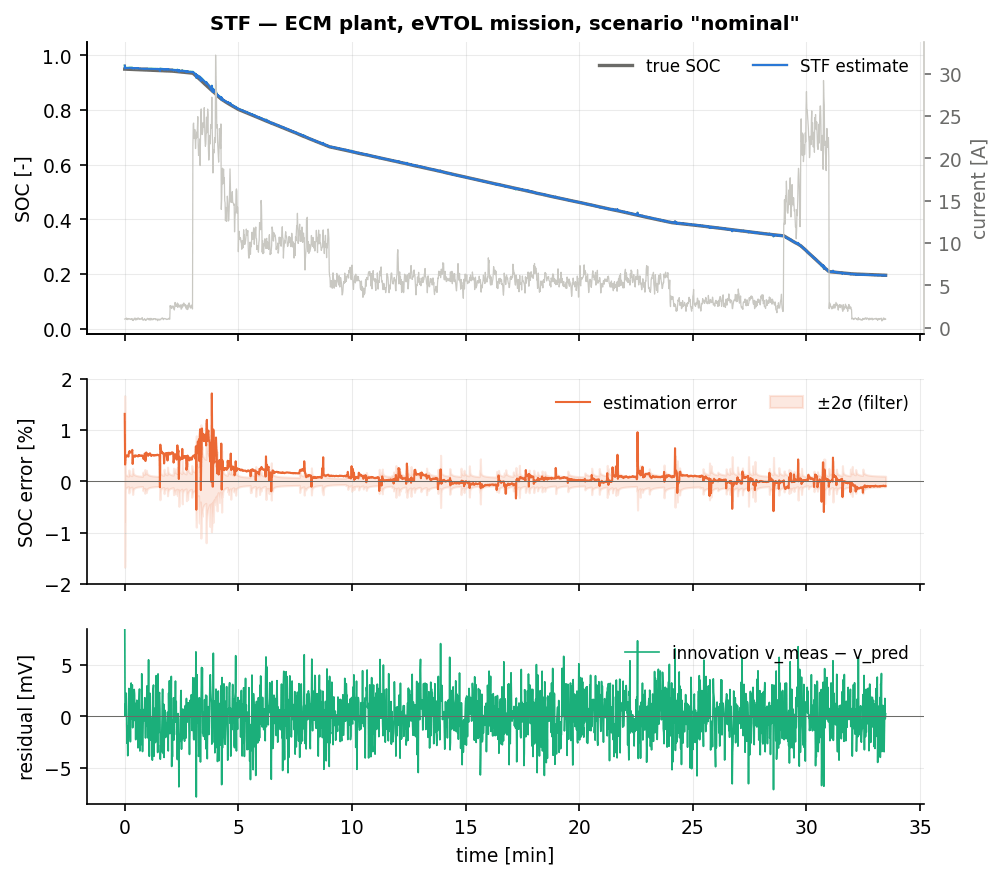
\includegraphics[width=\textwidth]{figures/cell_STF_nominal.png}
\caption{STF on the nominal eVTOL mission: true and estimated SOC (top), estimation error with the $\pm 2\sigma$ band when available (middle), voltage residual (bottom).}
\end{figure}
\begin{figure}[H]\centering
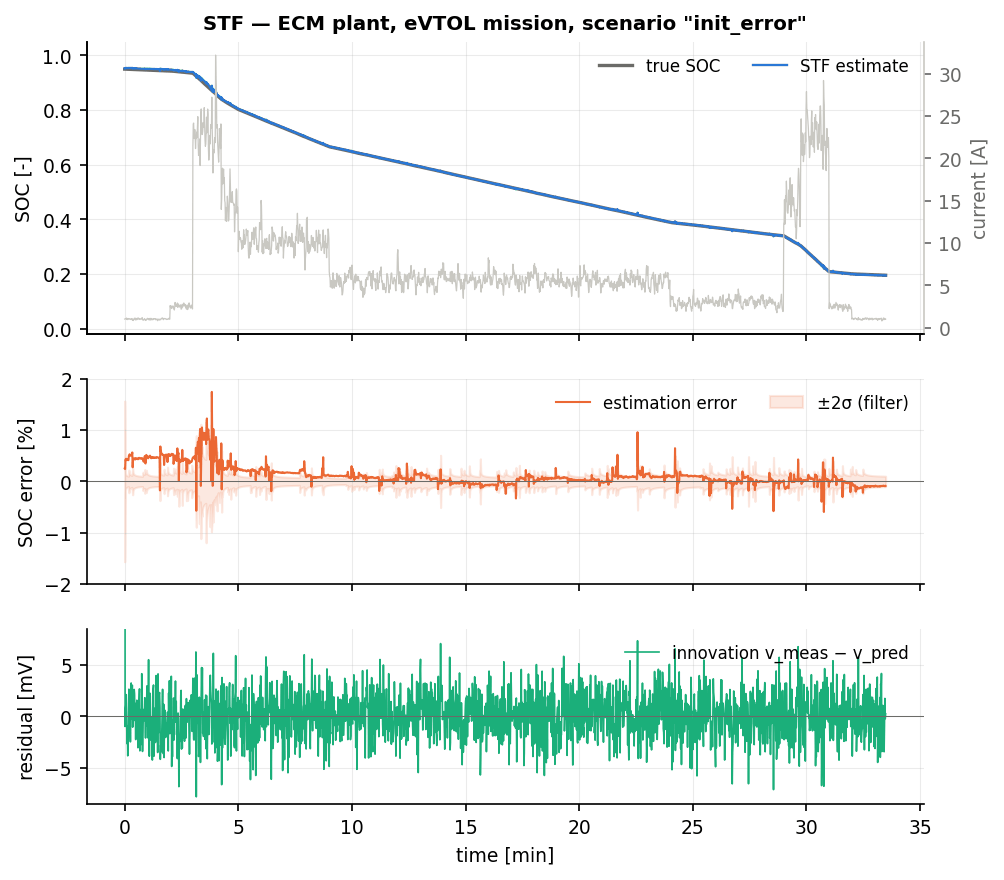
\includegraphics[width=\textwidth]{figures/cell_STF_init_error.png}
\caption{STF with a 35\,\% initial SOC error.}
\end{figure}
\begin{figure}[H]\centering
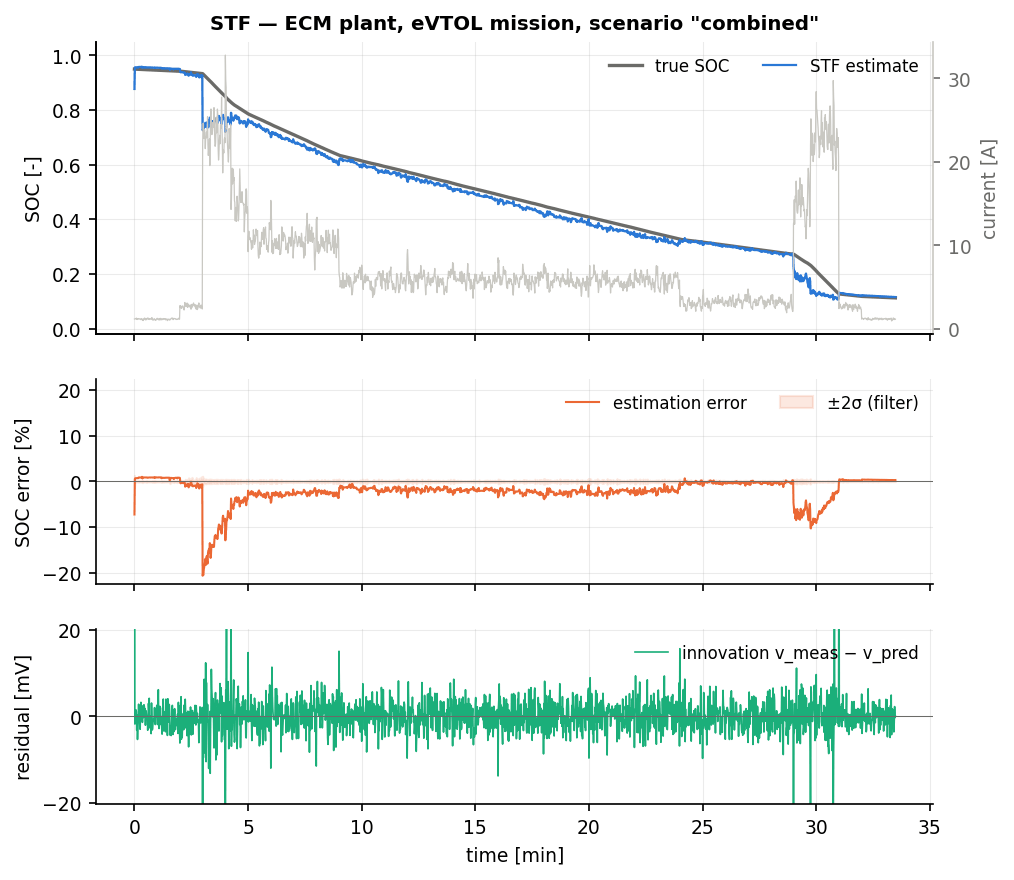
\includegraphics[width=\textwidth]{figures/cell_STF_combined.png}
\caption{STF on the \texttt{combined} scenario (25\,\% initial SOC error, \SI{150}{\milli\ampere} current bias, 2\,\% gain error, 10\,\% capacity loss with the associated resistance growth).}
\end{figure}
\begin{figure}[H]\centering
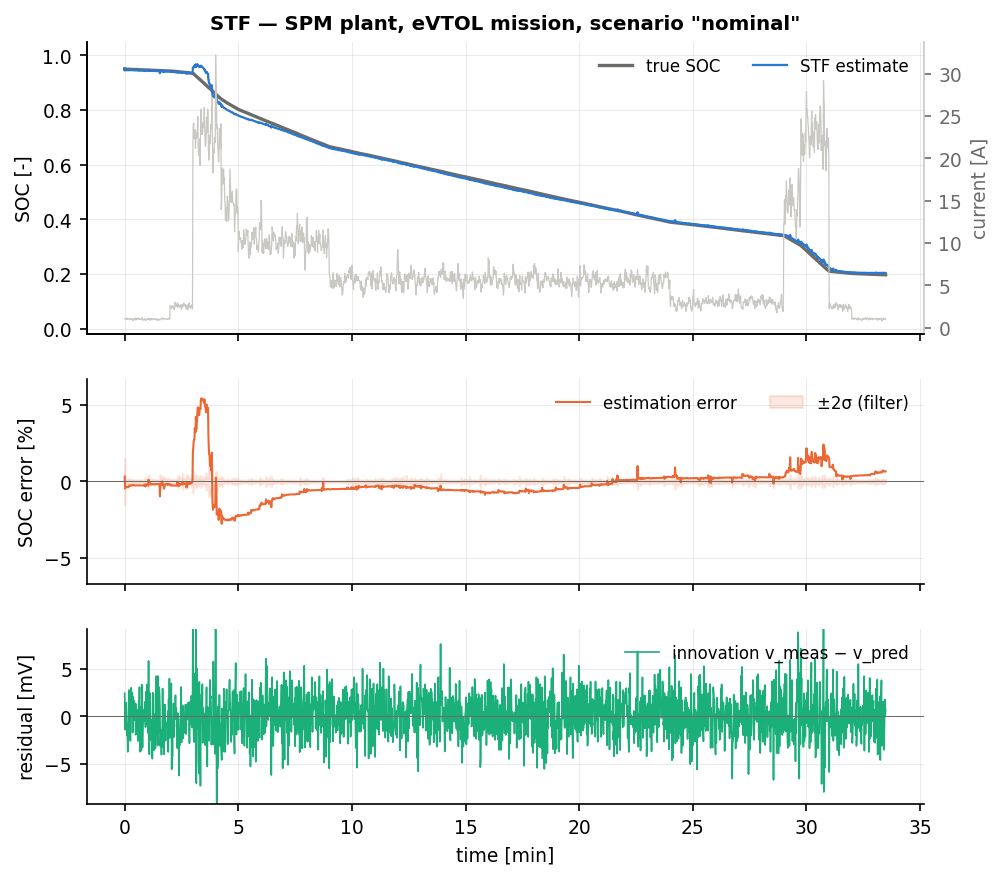
\includegraphics[width=\textwidth]{figures/cellspm_STF_nominal.png}
\caption{STF on the electrochemical (single-particle) plant, nominal mission: the estimator uses a 2-RC ECM fitted to that plant and therefore sees a structured \SI{4}{\milli\volt} residual instead of white noise.}
\end{figure}

All figures below are three-seed means in \% SOC, as tabulated above; the plain \texttt{EKF} run on
the same data is the reference (\texttt{EKF ref.} column).  For orientation, the EKF scores
$\mathrm{rmse}_{ss}$ = 0.05\,\% on \texttt{nominal}, 0.12\,\% on \texttt{noise\_step}, 0.21\,\% on
\texttt{outliers}, 0.46\,\% on \texttt{sensor\_dropout}, 1.36\,\% on \texttt{param\_mismatch},
1.52\,\% on \texttt{aged\_cell} and 12.44\,\% on \texttt{combined} (where it never converges), and
3.73\,\% on the nominal SPM mission.

\paragraph{Benign scenarios.}  \texttt{nominal}: $\mathrm{rmse}=0.24\,\%$,
$\mathrm{rmse}_{ss}=0.10\,\%$ against the EKF's $0.15\,\%$ / $0.05\,\%$.  The STF is about twice as
noisy as the EKF when nothing is wrong, with a maximum error of $2.57\,\%$ against $1.07\,\%$;
$\lambda_k$ is $1$ most of the time but fires on the manoeuvre pulses of the eVTOL profile (the
$+30\,\%$, \SI{3}{\second} current transients), where the linearisation error briefly inflates the
innovations.  Both values are comfortably inside the $2\,\%$ acceptance bound.
\texttt{init\_error} converges at $t=\SI{0}{\second}$ with $0.22\,\%$ / $0.10\,\%$.

\paragraph{Target scenario \texttt{combined}.}  This is the case the method exists for: a $25\,\%$
initial SOC error, a \SI{150}{\milli\ampere} current-sensor bias, a $2\,\%$ gain error and a
$10\,\%$ capacity loss with the associated $25\,\%$ resistance growth.  The EKF \emph{never}
converges to the $2\,\%$ band ($t_\mathrm{conv}=$ --, $\mathrm{rmse}=16.02\,\%$,
$\mathrm{rmse}_{ss}=12.44\,\%$): its covariance has collapsed, the \SI{16}{\milli\volt} voltage bias
produced by the grown $R_0$ is converted into a $12\,\%$ SOC error by the very flat OCV curve near
$\soc=0.9$, and it has no mechanism to notice.  The STF converges at $t=\SI{0}{\second}$ and holds
$\mathrm{rmse}=3.50\,\%$, $\mathrm{rmse}_{ss}=2.71\,\%$ --- a $4.6\times$ reduction of the full-run
RMSE and, more importantly, a qualitative change from "never converges" to "converges immediately".
The fading factor is doing exactly what it was designed to do: averaged over the first
\SI{200}{\second} (seed 1) $\lambda_k=8.6$, settling to $2.9$ over $[200,1000]\,\si{\second}$ and
$3.2$ over $[1000,2010]\,\si{\second}$, i.e.\ the filter permanently runs with about three times the
propagated covariance an ordinary EKF would use, which is enough to keep the gain from collapsing.
Its voltage prediction on this scenario is also the best in the family, $\mathrm{rmse}_v =
\SI{3.01}{\milli\volt}$ against the EKF's \SI{5.15}{\milli\volt} and the $\mR$-adapting filters'
\SI{14}{\milli\volt}--\SI{17}{\milli\volt}: inflating $\mP$ keeps the filter following the
measurement instead of abandoning it.

\paragraph{Other mismatch scenarios.}  \texttt{sensor\_dropout}: $\mathrm{rmse}$ $0.72\to0.49\,\%$,
$\mathrm{rmse}_{ss}$ $0.46\to0.10\,\%$ ($1.5\times$ / $4.6\times$) --- the frozen sensor produces
exactly the correlated innovation sequence the orthogonality test is looking for, although the
transient costs a maximum error of $8.63\,\%$ against the EKF's $2.27\,\%$.  On
\texttt{param\_mismatch} and \texttt{aged\_cell}, however, the STF is clearly \emph{worse} than the
EKF ($2.37\,\%$ / $1.84\,\%$ against $1.28\,\%$ / $1.36\,\%$, and $3.61\,\%$ / $2.68\,\%$ against
$1.18\,\%$ / $1.52\,\%$).  The reason is instructive: in both, the dominant model error is a
\emph{voltage} bias (wrong $R_0$), so inflating $\mP$ makes the filter trust the biased measurement
\emph{more}, and the SOC estimate is pulled further off.  The correct response there is to inflate
$\mR$, which is what the filters of \cref{ch:sagehusaakf}, \cref{ch:iaeakf} and \cref{ch:vbakf} do
--- and they achieve $0.76\,\%$--$1.30\,\%$ on those same scenarios.  \texttt{preisach} is the third
regression and the numbers moved with the corrected hysteresis sign convention: the STF now scores
$1.13\,\%$ / $0.98\,\%$ with $t_\mathrm{conv}=\SI{228}{\second}$ against the EKF's $0.58\,\%$ /
$0.20\,\%$ at \SI{16}{\second}, a factor of five worse, because a genuine un-modelled hysteresis
voltage is again an output-side error.  \texttt{cold} ($0.36\,\%$ against $0.16\,\%$) and
\texttt{current\_bias} ($0.84\,\%$ against $0.61\,\%$) are mildly worse for the same reason.

\paragraph{Where it must not be used.}  On \texttt{noise\_step} the STF is the worst estimator in the
family: $\mathrm{rmse}=1.94\,\%$, $\mathrm{rmse}_{ss}=2.34\,\%$ against the EKF's $0.18\,\%$ /
$0.12\,\%$, a factor of $20$ worse, with $\mathrm{rmse}_v$ rising to \SI{16.04}{\milli\volt}.  This is
the structural ambiguity of \eqref{eq:stf:cond} in its purest form: the tenfold rise of the
voltage-sensor noise at $t=\SI{600}{\second}$ inflates $\bm{V}_k$ by a factor of $\approx90$, the STF
reads that as model error, drives $\lambda_k$ to its covariance-cap-limited maximum, and the filter
ends up performing something close to an instantaneous OCV inversion of a \SI{20}{\milli\volt}-noisy
voltage.  \texttt{outliers} fails the same way ($1.44\,\%$ / $1.38\,\%$ against $0.52\,\%$ /
$0.21\,\%$) and is the only ECM scenario in this family where the STF does not reach the $2\,\%$ band
for \SI{60}{\second} ($t_\mathrm{conv}=$ --; no divergence).  If the sensor noise level is not known
to be constant, the STF must be combined with an $\mR$ estimator --- which is precisely the
fuzzy-supervised STF of \cite{jwo2007fuzzy} --- or replaced by an IMM (\cref{ch:imm}) that carries
both hypotheses explicitly and gets $0.05\,\%$ on \texttt{noise\_step} and $1.02\,\%$ on
\texttt{combined}.

\paragraph{Cost.}  \SI{532}{\nano\second}/step against the EKF's \SI{478}{\nano\second}/step, with no
buffers.

\paragraph{Electrochemical (SPM) plant.}  Here the picture inverts completely, and the SPM rows are
the strongest argument in this chapter for the method.  With a 2-RC ECM fitted to the single-particle
plant the residual is a structured, slowly varying \SI{4}{\milli\volt} signal --- genuine model error,
not sensor noise --- and that is exactly the hypothesis the orthogonality condition
\eqref{eq:stf:r2} is built on.  The STF reaches $\mathrm{rmse}_{ss}=\mathbf{0.66\,\%}$ on the nominal
SPM mission against the EKF's $3.73\,\%$, a $\mathbf{5.7\times}$ improvement, and against
$3.02\,\%$--$3.33\,\%$ for all four $\mR$-adapting filters, which improve on the EKF by barely
$10$--$20\,\%$.  The explanation is the one the ECM rows hinted at, seen from the other side.
Covariance matching cannot ask \emph{why} the residuals are large; concluding "noisy sensor" and
lowering the gain hands SOC to the coulomb integrator, and on this plant the integrator is the faulty
component (the fitted capacity and efficiency do not reproduce the true lithium inventory), so the
estimate parks at a $3\,\%$ offset.  The measurement is the reliable part --- the ECM's
$\ocv(\soc)$ map \emph{was} fitted to this plant --- so the useful response is to shorten the
filter's memory until recent measurements outweigh the accumulated model, which is what
$\lambda_k>1$ does.  Under structured model error, inflating $\mP$ (trusting the measurement more)
beats inflating $\mR$ (trusting it less), and the ECM \texttt{aged\_cell} row above is the mirror
image: there the error lived in the output map, and the ordering of the two families reverses.  The
advantage carries across the SPM scenarios --- \texttt{init\_error} $3.81\to0.66\,\%$,
\texttt{current\_bias} $5.69\to0.72\,\%$ ($7.9\times$), \texttt{sensor\_dropout} $5.31\to0.66\,\%$
($8.0\times$), \texttt{hot} $2.16\to0.74\,\%$, \texttt{param\_mismatch} $3.13\to1.75\,\%$ --- with the
two familiar exceptions where the disturbance really \emph{is} on the sensor: SPM
\texttt{noise\_step} ($2.53\,\%$ against $3.30\,\%$, an improvement but far behind Fading-EKF's
$0.43\,\%$) and SPM \texttt{outliers} ($1.64\,\%$ against $1.99\,\%$, $t_\mathrm{conv}=$ --).  SPM
\texttt{cold} is the one genuine failure ($5.12\,\%$ against $7.35\,\%$ in steady state but a
\SI{966}{\second} convergence time and a $17.88\,\%$ maximum error): at \SI{-10}{\celsius} the
diffusion time constant grows beyond \SI{2000}{\second}, the innovation sequence is correlated over
the whole mission, and the fading factor stays large enough to make the estimate jumpy.

\section{Summary}
The strong tracking filter adds one scalar to the EKF and buys a qualitative improvement in
re-convergence after model mismatch: on the hardest scenario of this benchmark it turns "never
converges, $12\,\%$ steady-state SOC error" into "converges immediately, $2.7\,\%$".  Use it when the
plant model is the suspect part and the sensor model is trustworthy --- manoeuvre changes, ageing,
parameter drift, stuck sensors.  Do not use it when the measurement-noise level itself can change,
because the orthogonality condition cannot tell the two apart and the filter will respond to a
noisier sensor by trusting it more.  Its best case in this benchmark is the electrochemical plant, where the 2-RC model leaves a
structured \SI{4}{\milli\volt} residual and the STF reaches $0.66\,\%$ against the EKF's
$3.73\,\%$ --- a $5.7\times$ gain, while every $\mR$-adapting filter manages only $10$--$20\,\%$,
because under model error the right move is to trust the measurement more, not less.  Never use it
without a covariance bound on a plant with weakly observable states: the scalar inflation is blind to
observability, and on this cell model the unbounded version reaches NaN in under \SI{200}{\second}.
